\documentclass[11pt, oneside]{article}   	% use "amsart" instead of "article" for AMSLaTeX format
\usepackage{geometry}                		% See geometry.pdf to learn the layout options. There are lots.
\geometry{letterpaper}                   		% ... or a4paper or a5paper or ... 
%\geometry{landscape}                		% Activate for for rotated page geometry
%\usepackage[parfill]{parskip}    		% Activate to begin paragraphs with an empty line rather than an indent
\usepackage{verbatim}
\usepackage{color}
\usepackage{graphicx}				% Use pdf, png, jpg, or eps� with pdflatex; use eps in DVI mode
								% TeX will automatically convert eps --> pdf in pdflatex		
\usepackage{amssymb}
\usepackage{graphicx}
\usepackage{listings}
\usepackage{longtable}
\usepackage[titletoc]{appendix}		% titletoc adds 'Appendix' before the letter in the TOC
\usepackage{hyperref}

 
\definecolor{dkgreen}{rgb}{0,0.6,0}
\definecolor{gray}{rgb}{0.5,0.5,0.5}
\definecolor{mauve}{rgb}{0.58,0,0.82}
 
\lstset{ %
  language=Octave,                % the language of the code
  basicstyle=\footnotesize,           % the size of the fonts that are used for the code
  numbers=left,                   % where to put the line-numbers
  numberstyle=\tiny\color{gray},  % the style that is used for the line-numbers
  stepnumber=2,                   % the step between two line-numbers. If it's 1, each line 
                                  % will be numbered
  numbersep=5pt,                  % how far the line-numbers are from the code
  backgroundcolor=\color{white},      % choose the background color. You must add \usepackage{color}
  showspaces=false,               % show spaces adding particular underscores
  showstringspaces=false,         % underline spaces within strings
  showtabs=false,                 % show tabs within strings adding particular underscores
  frame=single,                   % adds a frame around the code
  rulecolor=\color{black},        % if not set, the frame-color may be changed on line-breaks within not-black text (e.g. commens (green here))
  tabsize=2,                      % sets default tabsize to 2 spaces
  captionpos=b,                   % sets the caption-position to bottom
  breaklines=true,                % sets automatic line breaking
  breakatwhitespace=false,        % sets if automatic breaks should only happen at whitespace
  title=\lstname,                   % show the filename of files included with \lstinputlisting;
                                  % also try caption instead of title
  keywordstyle=\color{blue},          % keyword style
  commentstyle=\color{dkgreen},       % comment style
  stringstyle=\color{mauve},         % string literal style
  escapeinside={\%*}{*)},            % if you want to add LaTeX within your code
  morekeywords={*,...}               % if you want to add more keywords to the set
}


\title{Dimple Developer Documentation}
%\date{}							% Activate to display a given date or no date


\begin{document}


\maketitle

\clearpage
%\renewcommand{\contentsname}{Contents}
\setcounter{tocdepth}{3}				% Include paragraphs and subparagraphs in TOC
\tableofcontents

\clearpage

\section{Scope}

This document provides information about Dimple that will be useful to developers of Dimple.  Although fairly out of date, it still contains information useful for adding features to Dimple. 

This document contains: 

\begin{enumerate}
\item Unreleased Dimple Functionality - Describe at a high level what problems Dimple is meant to solve.
\item Thoughts about possible future Dimple functionality.
\item Dimple Architecture and Design - Provides details of the design for internal developers and patents. 
\end{enumerate}


\section{Dimple Functionality}

Dimple is intended as a tool for quickly prototyping algorithms that can be described with Factor Graphs.  In its current form Dimple provides ``clients'' and ``solvers''.  Users create Factor Graphs using the clients and then perform inference using the solvers.  There is currently a MATLAB and Java client.  Dimple is a set of classes and function calls and so MATLAB Dimple client code is similar to but not compatible with Java Dimple client code.  Both the MATLAB and Java Dimple clients can use the same Java solver but currently only the MATLAB client can use the C++ solver. 

Specific features

\begin{itemize}
\item Existing 
\begin{itemize}
\item See `Dimple User Documentation.pdf'
extended with new user created solvers.
\item Multiple methods of specifying schedules.
\item Specify arbitrary function node implementations - It might be valuable for users to override the Function Node implementation.  (To simulate hardware non-idealities)....
\item Debugging support - Dimple provides ways to view the messages and information about each factor and variable.
\item Multiple Solvers - Dimple currently provides SumProduct, MinSum, Gibbs, and other solvers.
\item Continuous Variables - Dimple has some support for continuous variables.
\end{itemize}
\end{itemize}

\section{Detailed API Documentation}

See `DimpleUserDocumentation.pdf'


\section{Architecture}


\subsection{High Level}

Dimple currently provides both a MATLAB and Python client.  Coding with MATLAB allows users access to MATLAB's data visualization tools, communications libraries, vector/matrix support, and general familiarity for hardware designers.  Coding in Python allows integration with FADL.

An early prototype of Dimple was written entirely in MATLAB.  This prototype's performance was suboptimal.  As a result Dimple is now architected so that the user interface is MATLAB or Python while the internals are implemented using C++ or Java.

Among the existing solvers are:

\begin{itemize}
\item Java Solvers - There are java implementations of multiple solvers (including sum product, min sum, and gibbs).  These are the most feature rich of all the solvers.
\item Python Solver - This solver is less flexible than the Java solvers.  It is at least 10x slower than the Java solver but is useful when performance is not an issue and Jython cannot be used.
\end{itemize}

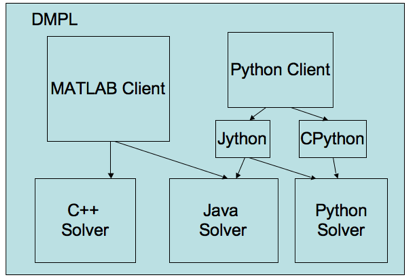
\includegraphics{images/DimpleHighLevelArchitecture.png}

Users develop programs as described in the user manual section of this document.  Their programs can refer to user created delta functions or pre-made delta functions residing in the Dimple/lib directory (if Dimple is installed correctly)

When executed, the user's program makes calls to MATLAB functions provided by the Dimple installation. Dimple uses some MATLAB OOP features, so user defined Variables, Graphs, and Graph Definitions are all represented by MATLAB classes.

\subsection{Detailed Architecture}

\subsubsection{Factor Graphs and the Sum-Product Algorithm}

Before describing the Java, Python and MATLAB architecture in more detail it is probably useful to describe some of the details of the Sum-Product algorithm here.  The two references at the beginning of this document provide more detail on the Sum-Product algorithm and are probably necessary reading to put the following descriptions in context.

As either of the references will mention, Factor Graphs are bipartite graphs of Variable Nodes and Function Nodes.  The bipartite-ness means that there are two sets of nodes (in this case Variable and Function) and nodes from one set connect only to nodes of the other set.

The optimal scheduling of the Sum-Product algorithm on trees is understood and well defined but Dimple supports loopy graphs (our LDPC is a loopy graph) and the optimal scheduling on loopy graphs is not well understood.  Dimple provides multiple schedulers as well as hooks for developing new schedulers.  Existing schedulers include TreeAndFloodingScheduler which will pick an optimal schedule for a tree graph or a flooding schedule for a non tree graph.

Let's now examine how messages are computed for Function and Variable nodes.

\paragraph{Function Nodes}

Because Dimple currently only supports discrete m-ary variables (where m is finite), messages are simply double arrays where the elements of the array sum to 1 and map to elements of elements in the variable's domain.  The messages are really PMFs (Probability Mass Functions) of the variables' domains.  

The following equation can be used to describe how to compute one element of the Msg array for a given edge. 

\[
 p(X=x) = \sum_y \sum_z \delta (X=x,Y=y,Z=z)p(y)p(z) 
 \]

In this case, we have a function node connected to three variables: X, Y, and Z.  We are computing the probability that X=x.  We marginalize over all possible Ys and Zs.  The delta function will return 1 (or any other positive real value) for all valid combinations of X,Y, and Z.

The following pseudo-code implements that math:

\begin{lstlisting}
For each value of X
   p(X=x) = 0;
    For each combination of Y and Z
      If (x,y,z is legal combination)
        p(X=x) = p(X=x) + p(y)*p(z)
      End
   End
End
\end{lstlisting}


\paragraph{Equals Nodes}

Equals nodes are similar to function nodes but can be simplified as follows:

Math for equals update

\[
 p(X_1=x) = p(X_2=x)*p(X_3=x) 
 \]

In addition, at the end of the Sum-Product algorithm, users read the beliefs of the variable nodes of interest.  These beliefs take into account the inputs as well as all attached function nodes.

Math for equals belief:


\[
 p(X=x) = input(X=x)*p(X_1=x)*p(X_2=x)*p(X_3=x) 
 \]

\paragraph{Tables}

Looking at the Function Node pseudo-code you can see the line that says ``for each combination of Y and Z''.  Legal combinations can be discovered using Delta Functions provided by the user.  

In the case of the XOR, the Delta function can be written:

\begin{lstlisting}
Function valid = xorDelta(array)
	 valid = 1;
	 for i =1:length(array)
 	     valid = bitxor(valid,array{i})
	     end
end
\end{lstlisting}

It can be noted that all delta functions can be represented as tables.  If we examine the XOR function with three bit binary inputs we get the following table:

\begin{tabular}{ c | c | c | c}
 x & y & z & Valid \\
\hline
 0 & 0 & 0 & 1 \\
0 & 0 & 1 & 0 \\
 0 & 1 & 0 & 0 \\
 0 & 1 & 1 & 1 \\
 1 & 0 & 0 & 0 \\
 1 & 0 & 1 & 1 \\
 1 & 1 & 0 & 1 \\
 1 & 1 & 1 & 0 \\
\end{tabular}

If you look at the function node pseudo-code again, you will see that all non-valid entries result in NOPs, so we can compress the table to:

\begin{tabular}{ c | c | c | c}
 x & y & z & Valid \\
\hline
 0 & 0 & 0 & 1 \\
 0 & 1 & 1 & 1 \\
 1 & 0 & 1 & 1 \\
 1 & 1 & 0 & 1 \\
\end{tabular}

In order to minimize the number of computations, we generate the tables for all Delta Functions before running the Sum-Product algorithm.

Now let's get into the actual architecture.



\subsubsection{Client/Modeler/Solver Architecture}


Dimple now supports a Java client in addition to the MATLAB and Python clients.  The architecture for each version has three high level layers: 


\begin{itemize}
\item Client - These classes provide the UI and exist to hide unwanted details from the user.
\item Model - The model layer is separated from the Solver layer so that users can build Factor Graphs and switch the solver without rebuilding their model.  The model layer should contain a  description of the connectivity of the graph, the combo tables, be able to store priors, etc...
\item Solver - The solver layer implements the solve function, should take the graph, the inputs and produce beliefs.  A sumproduct solver will perform the Sum Product algorithm using BP.
\end{itemize}


In Java, we have a Client, Model, and Solver layer.  In addition we have a MATLAB proxy layer which exists to provide any features the MATLAB client expects that the Java Client does not implement.  VariableVectors are an example of such a feature.

The MATLAB Dimple client can be connected to multiple Model Factories.  There is currently just one such factory right now: the Java MATLAB proxy layer and instantiates Java MATLAB Proxy classes.

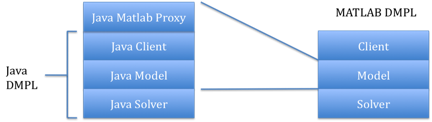
\includegraphics{images/ArchitectureLayers.png}


\subsubsection{Java Solver}

\paragraph{Client, Model, and Solver relationships}

Let's now examine the MATLAB architecture when using a MATLAB client and Java Model and Solver.  The following graph is a simplified view of some of the class relationships.

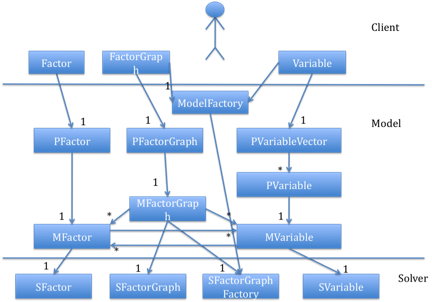
\includegraphics{images/DetailedLayers.png}
 
The user interacts with the Client layer, which mostly consists of the FactorGraph, Variable, and Factor classes.  Both FactorGraphs and Variables retrieve a global ModelFactory object using the getModeler() function.  The ModelFactory object can be changed with the setModeler() function.  The architecture assumes that all Variables added to a FactorGraph will share the same ModeleFactory.

All of the MATLAB classes contain pointers to corresponding Model classes.  The ModelFactory is responsible for instantiating the Model objects for FactorGraph and VariableVector.  In the diagram, these classes are called PFactorGraph and PVariableVector.  The P stands for Proxy.  The Java code provides a set of MATLAB proxy classes, which inherit from the Java client's classes.  The proxy layer is necessary to provide  the appropriate methods for the MATLAB interface without cluttering the Java client.

PFactor, PFactorGraph, and PVariable are all thin wrappers around the Java MFactor, MFactorGraph, and MVariable classes.  These classes provide the connectivity of the graph.  The MFactorGraph class contains a Scheduler and ultimately a schedule.  Schedules will describe the order that nodes and edges should be updated.  

When the SolverFactory is passed to the FactorGraph, the FactorGraph will create Solver objects for each Factor Graph, Variable, and Factor.  When the Factor Graph's solve method is called, the MFactorGraph class iterates the schedule and calls update on all of the objects provided by the schedule.  The update function on the Model objects is passed down to the solver objects.  

\paragraph{Relationship between Model and Solver}

The Model Variables and Factors contain Ports which connect to other nodes as well as input messages:

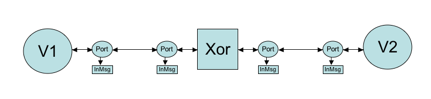
\includegraphics{images/PortsAndNodes.png}
 
Even though the Model objects contain the connectivity and messages, the Solver is responsible for initializing and updating the messages.  This architecture was chosen to allow solvers to be as simple as possible while still making the solvers responsible for performing the solve algorithm.

\paragraph{Object instantiation}

Users are responsible for creating FactorGraphs, Variables, the ModelFactory and the FactorGraphFactory.  Dimple provides defaults for the ModelFactory and FactorGraphFactory.  The following diagram provides red arrows showing how each object is instantiated.  Blue arrows indicate containment. 

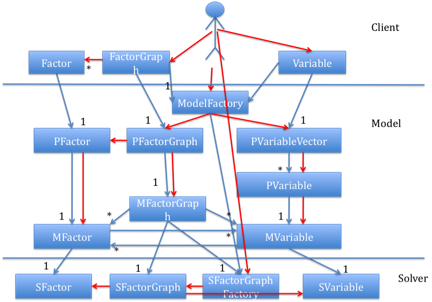
\includegraphics{images/ObjectInstantiation1.png}

The user calls: 

\begin{lstlisting}
fg = FactorGraph
\end{lstlisting}

\begin{enumerate}
\item FactorGraph object is created
\begin{enumerate}
\item It calls getModeler to get the ModelFactory
\begin{enumerate}
\item If no modeler is already set, it will create a default Modeler and then call setSolver on theModelFactory using the getSolver function.  
\end{enumerate}
\item It calls createGraph on the ModelFactory to create the PFactorGraph object
\begin{enumerate}
\item When the PFactorGraph object is created it instantiates an MFactorGraph object.
\item It passes the ModelFactory's Solver (SolverFactory) to the newly created MFactorGraph.  Although the architecture is meant to allow Models to exist without Solvers, it also ensures the Model is setup with a default Solver so that users don't have to explicitly set a Solver.
\item The MFactorGraph setSolverFactory method will store the SolverFactory and also call createFactorGraph and store the SFactorGraph object that was created as a result of that call.
\end{enumerate}
\end{enumerate}
\end{enumerate}

At this point we have:

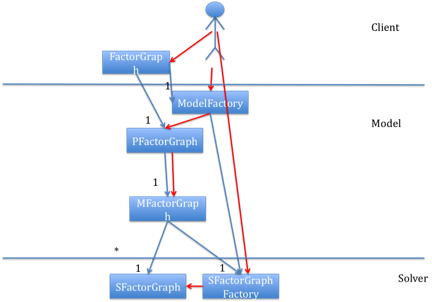
\includegraphics{images/ObjectInstantiation2.png}

Next, the user can call:

\begin{lstlisting}
b = Bit(3,1);
\end{lstlisting}

\begin{enumerate}
\item Bit and Variable both inherit from VariableBase.  The object diagram hides this complexity and represents this entire class structure with a single ``Variable'' box.
\item The VariableBase class calls getModeler()
\item It calls createVariableVector on the resulting ModelFactory
\begin{enumerate}
\item The PVariableVector creates N PVariableVectors
\begin{enumerate}
\item The PVariableVector is attached to an MVariableVector
\end{enumerate}
\end{enumerate}
\end{enumerate}

Now we have:

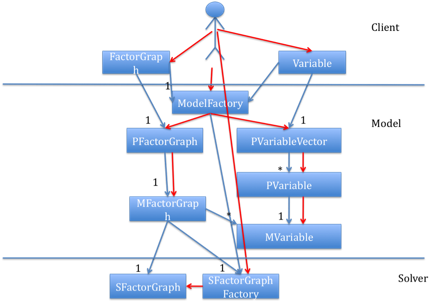
\includegraphics{images/ObjectInstantiation3.png}

Note that the MVariable doesn't have an underlying Solver object yet.

Next the user can call:

\begin{lstlisting}
f = fg.addFactor(@xorDelta,b);
\end{lstlisting}



\begin{enumerate}
\item First we should note some architectural details not mentioned in the object diagram.  First, MATLAB provides both a Factor and TableFactor class.  The TableFactor class inherits from Factor and assumes that the Factor has a combination table.  Second, if a solver does not provide a custom factor, the Factor Graph will generate a combination table for each unique set of function handles and argument domains it encounters.  Currently there is a one to one mapping of FactorGraphs to CombinationTableFactories.  The CombinationTableFactory is responsible for generating combo tables as well as caching combo tables.
\item FactorGraph calls customFactorExists on the PFactorGraph object.  This call is passed down to MFactorGraph and MFactorGraph returns false if no solver is set and otherwise passes the call down to SFactorGraph.  The Solver is responsible for returning true only in cases where it actually has a hand coded implementation of the specified factor.
\item If a custom factor exists
\begin{enumerate}
\item createCustomFactor is called on the PFactorGraph object.
\begin{enumerate}
\item This object calls createCustomFactor on the MFactorGraph object


\begin{enumerate}
\item This object creates an MFactor object and provides it the name that was passed down the call chain
\item It then calls attach on this object, passing it the FactorGraph solver



\begin{itemize}
\item The MFactor object attach call will call createCustomFactor on the FactorGraph Solver


\begin{itemize}
\item This method is responsible for instantiating a solver object that corresponds to the custom factor.  For instance, the SumProduct Solver supports a FiniteFieldPlus class to handle an addFactor(@finiteFieldPlus,vars) call.
\end{itemize}
\end{itemize}
\end{enumerate}
\item The PFactorGraph will wrap this object in a PFactor instance
\end{enumerate}
\item The FactorGraph object will wrap this object in a Factor instance.
\end{enumerate}
\item If a customFactor does not exist
\begin{enumerate}
\item The FactorGraph class calls getComboTable on the CombinationTable factory.
\begin{enumerate}
\item This method will look to see if a combo table exists for the specified function handle and domainlist.  If it does not, it will create the combo table by calling the function handle for each combination of domain elements of the argument list. 
\end{enumerate}
\item If the combo table is new, the FactorGraph class calls createTable on the PFactorGraph object.  This object calls create Table on MFactorGraph which then stores the table in a hashtable using an ID as the key.
\item The FactorGraph class calls createTableFactor on the PFactorGraph object
\begin{enumerate}
\item PFactorGraph calls createTable on MFactorGraph
\begin{enumerate}
\item MFactorGraph retrieves the table by its id
\item It creates an MTableFactor
\item It calls attach on all of the MVariables involved in the Factor
\begin{itemize}
\item The MVariable attach function tells the FactorGraphSolver to instantiate a Variable Solver object and stores a pointer to this object.
\end{itemize}
\item It calls attach on the MTableFactor object.
\begin{itemize}
\item The MTableFactor object tells the Solver to create a TableFactor object and attaches to this.
\end{itemize}
\end{enumerate}
\item It wraps this object in a PTableFactor object.
\end{enumerate}
\item FactorGraph wraps the returned object in a TableFactor object.
\end{enumerate}
\end{enumerate}



At this point, the entire object model (with the exception of scheduler objects) has been created.  All solver objects exist.

The user executes:

\begin{lstlisting}
fg.NumIterations = 1
\end{lstlisting}

\begin{enumerate}
\item This results in FactorGraph calling setNumIterations on PFactorGraph, which calls setNumIterations on MFactorGraph, which then stores the number of iterations.
\end{enumerate}

The user executes:

\begin{lstlisting}
fg.solve();
\end{lstlisting}



\begin{enumerate}
\item FactorGraph calls solve on PFactorGraph which calls solve on MFactorGraph
\begin{enumerate}
\item MFactor graph throws an error if the solver is not set
\item MFactorGraph calls solve on SFactorGraph
\item If the Solver inherits from SFactorGraphBase it can use the following default implementation
\begin{enumerate}
\item Call initialize on the MFactorGraph object
\begin{enumerate}
\item Go through each MFactor and call initialize
\item Tells the solver object to initialize all the ports messages
\item Tells the solver object to initialize itself
\end{enumerate}
\item Go through each MVariable and call initialize
\begin{enumerate}
\item Does the same thing as the MFactor initialize.
\end{enumerate}
\item Go through each nested graph and call initialize
\end{enumerate}
\item Call iterate with the number of iterations
\begin{enumerate}
\item Iterate calls update and also calls sleep to allow for interrupts
\begin{enumerate}
\item Update calls getSchedule on MFactorGraph
\begin{itemize}
\item Calls createScheduleIfNeeded
\begin{itemize}
\item This method checks to see if the graph has changed or no schedule exists for this graph yet.
\item If the schedule needs to be updated
\item If there is a scheduler associated with this graph, that scheduler is asked to create a schedule
\item Otherwise, if there is a scheduler associated with the solver, ask that scheduler to create a schedule
\item Otherwise, ask the Default Scheduler (a singleton object) to create a schedule.
\item Different schedulers will use different algorithms to create a schedule.  A TreeOrFloodingScheduler will try to update the fewest number of edges possible if the graph is a tree and otherwise create a fixed flooding schedule.
\end{itemize}
\end{itemize}
\item It then calls update on every IScheduleEntry returned by the Schedule's iterator.
\begin{itemize}
\item The iterator's next function will return objects that implement the IScheduleEntry interface.  These will most likely be NodeScheduleEntry objects or EdgeScheduleEntry objects.  The former will call update on a Node (MVariable or MFactor) and the latter will call updateEdge on a Node.
\begin{itemize}
\item The MVariable or MFactor update will call update on the corresponding SVariable or SFactor node.  The solver nodes are responsible for reading the messages (retrieved from the MVariable and MFactor ports) and writing the messages (retrieved from the same place).
\end{itemize}
\end{itemize}
\end{enumerate}
\end{enumerate}
\end{enumerate}
\end{enumerate}



The user executes:

\begin{lstlisting}
b.Beliefs
\end{lstlisting}

\begin{enumerate}
\item The Variable class calls getBelief on the PVariableVector, which in turn calls getBelief on all of its contained PVariables.  The PVariables call getBelief on the MVariable which finally calls getBelief on the SVariable
\begin{enumerate}
\item The SumProduct SVariable class will retrieve the messages from the incoming ports of the MVariable object, perform the sum product belief calculation and return an array of doubles containing the answer.
\end{enumerate}
\end{enumerate}

\paragraph{Scheduler}

The previous section talks a bit about the scheduler.  The following is a class diagram showing the relationships between Scheduler, Schedule, and ScheduleEntries.

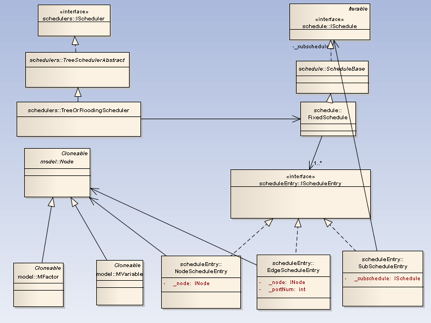
\includegraphics{images/Scheduler.png}

\subsubsection{Creating a new Solver}

Dimple provides a modular architecture which makes it relatively easy to create a new Solver.  To aid in the development of a new solver, Dimple provides a template located in the com.analog.lyric.dimple.solvers.template package.  Users can copy this template to speed up the creation of a new solver.

To create a new solver, simply create a new namespace "com.analog.lyric.dimple.solvers.\textless Package Name\textgreater. 

In this new package, the user has to create only four new classes:

\begin{itemize}
\item Solver - The Solver class must implement IFactorGraphFactory and can extend SolverBase. This class is responsible for instantiating SFactorGraph instances.
\item SFactorGraph - This class can extend SFactorGraphBase which, in turn, extends SNode and implements ISolverFactorGraph.  It is responsible for instantiating variables and factors.
\item SVariable - This class can extend SVariableBase or SDiscreteVariableBase.  Use the latter if your solver uses double arrays as messages.  The SVariable is responsible for calculating the variable message passing math. In addition it is responsible for initializing messages.
\item SFactor - The SFactor class can extend STableFactorDoubleArray, STableFactorBase, or SFactorBase. The template inherits from STableFactorDoubleArray.  This class is responsible for calculating the Factor message passing math.
\end{itemize}

Assuming com.analog.lyric.dimple.solvers.\textless Package Name\textgreater.Solver exists, users can  use the following to instantiate their new solver:

\begin{lstlisting}
fg = FactorGraph();
fg.Solver = '<Package Name>';
\end{lstlisting}

As long as their solver is in the correct namespace and on the java class path, MATLAB can instantiate the solver from the last portion of the namespace.

\subsubsection{Initializing solver state}

To understand how solver state is initialized and maintained, we look at several use cases.

\paragraph{User Sets Solver}

When the user sets the solver on the Factor Graph.  The factor graph creates solver objects and does a two way attachment from model to solver and vice versa.  When the variable solver objects are created, model properties are sent down to the variable solver objects.

Factor solver objects are created after all variable solver objects have been created.  As each factor solver object is created, it is told to create any needed messages.

The following is pseudo code describing this process:

\begin{lstlisting}
fg.setSolverFactory(IFactorGraphFactory factory)
	setSolverFactorySubGraph(factory)
		_solverFactory = facotry;
		_solverFactorGraph = factory.createFactorGraph(this)
			Instantiates the Solver Factor Graph
	for each variable
		var.createSolverObject(_solverFactorGraph)
			_solverVariable = factorGraph.createVariable(this);
				Decide what type of variable to create
				SomeVariableConstructor(var)
					_model = var;
					_var = var
			_solverVariable.createNonEdgeSpecificState()
				Create any state that is not specific to edges
			_solverVariable.setInput(_input)
				Tell the solver what the input is at this point in time
	for each nested graph
		ng.setSolverFactorySubGraphRecursive(factory)
			setSolverFactorySubGraph
			for each nested graph
				setSolverFactorySubGraphRecursive(factory)
	for each non graph factor
		f.createSolverObject(_solverFactorGraph)
			_solverFactor = factorGraph.createFactor(this)
				decide what kind of factor to create
				SomeFactorContructor()
					_factor = factor
					_model = factor
			_solverFactor.createMessages()
				//The following is for the sum product solver
				//more generally, make sure any messages needed are created
				initialize pointers to messages
				for each variable connected to the factor
					messages = varaibleSolver.createMessages(this);
						for the given factor, create the appropriate messages
						pass back the input and output messages
					cache the messages
	_solverFactorGraph.postSetSolverFactory()
		This gives the solver the opportunity to do any cleanup needed after the solver is set.
		The gibbs solver uses this opportunity to propagate fixedValues through the graph
		
\end{lstlisting}

\paragraph{User calls addFactor}

During this use case, the factor model object is creates.  Variables are added to the graph if they're not already part of the graph.  Variable solver objects are created and their non edge specific state is created.  Factor solver objects are created and they are told to create messages for each edge.

\begin{lstlisting}
fg.addFactor(factorFunction, Object ... vars)
	//For simplicity, let's assume there are no constants
	addFactorNoConstants
		for each variable
			setVariableSolver(v)
				if the solver has been set on this graph
					if the variable does not belong to this graph
						v.createSolverObject(_solverFactorGraph)
							This is documented in the previous use case
							In summary
								the solver object is created
								the object is told to create non edge specific state
								inputs and other model properties are passed down							
		if allDomainsAreDiscrete
			create new Factor
				assign factor function
				for each variable
					addVariable
						connects the variable to the factor and vice versa
		addFactor(factor,vars)
			for each variable
				make sure the variable is added to the list of variables of the graph
			set the factor's parent graph to this
			add the factor to this graphs list of factors.
			increment the versionId so that scheduling knows to recompute
		if the solver has been set on this graph
			f.createSolverObject(_solverFactorGraph)
				This is documented in the previous use case
				In Summary
					creates the solver object
					tells the solver object to create new messages
			_solverFactorGraph.postAddFactor(f);
				The solver can use this opportunity to do any cleanup once both the variable
					and factor solver objects have been created
				The Gibbs solver uses this opportunity to propagate the fixedValue

	
\end{lstlisting}


\paragraph{User changes inputs or other model property}

When the user sets a property on the model, the model saves that value but also passes it down tho the solver if the solver object exists.  If the solver is changed later, the model object will set that property on the solver after the new solver object is created.

TODO: How do we deal with FixedInput?  When new factors are added?  When the solver changes?

\begin{lstlisting}
var.setInputObject(value)
	_input = value
	if solver is set
		solver.setInput
			solver should do what it needs to do with inputs
\end{lstlisting}

\paragraph{User calls initialize}

Initialize is used to reset the messages in the solver.  This is usually invoked when solve is called so that the solver's original state is identical for each solve.

\begin{lstlisting}
fg.initialize()
	for each owned variable
		v.initialize()
			if solver exists, solver.initialize()
				for each edge
					resetEdgeMessages(edgeIndex)
						resetInputMessage 
						resetOutputMessage									
		if this is the root graph
			for each boundary variable
				v.initialize()
					same as before
		for each non graph factor at this level (don't descend)
			f.initialize()
				for each edge
					resetEdgeMessages
						NOP // for sum product
		for each nested graph
			g.initialize()
				//recursively initialize
			
		_solverFactorGraph.resetMessages()
	
\end{lstlisting}

\paragraph{User calls solve}

Solving ensures the solver is set, resets the messages if the user requests this, and runs through the schedule to update nodes in the sequence specified by the scheduler.  In addition, if this is a rolled up graph, it will advance messages, inputs,  save outputs, and recreate messages for the newest variables and factors (see the advance use case).

\begin{lstlisting}
fg.solve(init)
	checkSolverIsSet
		throw an error if it isn't
	_solverFactorGraph.solve(init)
		_factorGraph.initialize()
			See initialize use case
			Resets all messages
		solveOneTimeStep
			iterate(numIterations)
				//ignore multithreading for now
				for each iteration
					update()
						for each entry in the schedule
							entry.update()
								This will result in updating edges or nodes
								for variables, factors and nested graphs				
		continueSolve
			while the model has more data (assuming rolled up graphs)
				if the number of steps has been reached
					break
				getModel().advance()
					See advance use case
				solveOneTimeStep
					Same as before
					
		

\end{lstlisting}

\paragraph{advance}

Advance attempts to move all messages down the chain.  New state is recreated for the new variables and factors.  BlastFromThePast factors store messages from factors that disappear.  Input streams are applied.  Output streams get data from variables that fall off the ends.

\begin{lstlisting}

fg.advance()
	for each variable stream
		vs.advanceState()
			if there is a data sink
				//TODO: make this generic for other properties
				retrieve the belief from the first variable
				store it in the sink
			for each variable (not including the last)
				moveInputs on the modeler(from the next guy)
				//TODO Fixed input on the modeler?
				solver.moveNonEdgeSpecificState(from the next guy)
			for the last variable
				svar.createNonEdgeSpecificState()
					This is also called whenever a new solver object is created
					This gives the solver a chance to create any non edge specific
					stuff.
			if there is a data source
				on the last variable
					var.setInputObject(dataSource.next())
			else
				on the last var
					var.setInputObject(null)
			//TODO: what about Fixed input?			
	for each factor graph stream
		fgs.advance()
			for each parameter blast from the past handler
				handler.advance()
					for each blast from the past
						bfp.advance()
							for the var connected to the blast from the past
								var.moveMessages(otherPort)
									Move messages is responsible for moving
									messages from one node to this one.
			for each blast from the past chain
				for each blast from the past
					bfp.advance()
						same as above
			for each graph in the list of nested graphs
				nestedGraph.solver.moveMessages(next graph in the chain)
					for each factor
						sfactor.moveMesages(corresponding factor in other graph)
							for each edge
								moveMessages(other,edgeIndex,edgeIndex)
									Responsible for moving factor messages
								get connected variable
									svar.moveMessages(other var)
										responsible for moving var messages
					for each variable
						svar.moveNonEdgeSpecificState(corresponding var)			
							Responsible for moving all non edge specific state
			for the last nested graph
				graph.recreateMessages()
					for each variable
						svar.createNonEdgeSpecificState
							already documented
							Responsible for creating initial state
					for each factor
						sfactor.createMessages()
							//The following is for the sum product solver
							//more generally, 
							    make sure any messages needed are created
							initialize pointers to messages
							for each variable connected to the factor
								messages = varaibleSolver.createMessages(this);
								for the given factor, create the appropriate messages
								pass back the input and output messages
							cache the messages
			
	_solver.postAdvance()
		Give the solver the opportunity to update any state when advance occurs.
		The gibbs solver uses this opportunity to reset its best sample index

\end{lstlisting}



\subsubsection{LP and IP Solver}

\paragraph{How to express a Factor Graph as an LP or IP}

Inference on Factor Graphs can be expressed as a Linear Program or an Integer Program.  Expressed as an Integer program, inference will be exact but slower than BP.   The following math describes how to specify an objective function and constraints.

\subparagraph{Objective Function}

In the following, $F$ is the set of all factors and $V$ is the set of all variables.  $V_f$ is the set of all variables associated with factor $f$.  $\phi_f$ is the factor function for factor f.

\[
\sum_{f \in F} \phi_f(V_f) p(v) + \sum_{v \in V} input(v) p(v)
\]

\subparagraph{Constraints}

First we introduce some shorthand notation.  $ \sum_{\sim v} $ is a sum over all variables that are not v.  

For all pairs of f,v such that v is connected to f:

\[
\sum_{ \sim v} p(V_f) = p(v)
\]

also, for all v

\[
\sum_{v} p(v) = 1
\]

And finally

for all f

\[
p(V_f) \ge 0
\]

\subparagraph{Additional Constraint to Make this an IP}
When solving exactly, we make the previous equations an IP by constraining p(V=v) to be 0 or 1.

\subsubsection{Setting and Getting Properties on MATLAB Vectorized Objects}

Because looping in MATLAB is very slow, Dimple supports vectorized Factor, FactorGraph, and Variable objects.  This section discusses how getting and setting properties on these classes (which all inherit from MatrixObject) should behave.

We will discuss setting properties:

\begin{lstlisting}
a.b = c
\end{lstlisting}

a will always be a MATLAB object that inherits from the MatrixObject type.  MatrixObjects consist of a collection of underlying Java objects that inherit from the Node type.  c might be a MATLAB scalar, vector, matrix or tensor, a cell array, a MatrixObject, or a cell array of MatrixObjects.

We will also discussing getting properties:

\begin{lstlisting}
c = a.b
\end{lstlisting}

\paragraph{Numeric}

Somer properties take  and return numeric values.  For instance, discrete variable Node Belief and Input properties are arrays of numbers.  

\subparagraph{set}

When the underlying MatrixObject is a scalar, the dimension of a is [1 1].  This case is straightforward as c is simply passed on to the single Node.

\begin{lstlisting}
d = Discrete(0:2);
d.Input = ones(3,1);
d.Input = ones(1,3);
\end{lstlisting}

When a is a column vector, the size of a would be of the form [n 1].  The size of c will be [n y] where y can be a vector of numbers.  In the following case y = [3].  The a(i) Node will be assigned c(i,:);

\begin{lstlisting}
a = Discrete(0:2, 4, 1);
c = ones(4,3);
a.Input = c;
\end{lstlisting}

Here is another case where y = [2 3].  The a(i) Node will be assigned c(i,:,:);

\begin{lstlisting}
a = Discrete(0:2, 4, 1);
c = ones(4,2,3);
a.SomeProperty = c;
\end{lstlisting}

Finally, in the most general case where a is a row vector, matrix, or tensor, the size of a can be described by a vector x and the size of c can be described by a vector [x y] where x and y are both vectors.  When a.b is assigned c, each Node indexed by x will be assigned the tensor with dimensions y

Here is an example with a row vector:

\begin{lstlisting}
a = Discrete(0:2,1,4);
c = ones(1,4,3);
a.Input = c;
\end{lstlisting}

And an example with a tensor:

\begin{lstlisting}
a = Discrete(0:2,3,4,5);
c = ones(3,4,5,6,7);
a.SomeProperty = c;
\end{lstlisting}

In this case, each a(i,j,k) is assigned a 6x7 matrix.

\subparagraph{get}

In the case where a is a scalar and c is an array, c = a.b will return a column vector.  When c is a multi dimensional array, c = a.b will return the multidimensional array a a matrix or tensor.

In the case where a is a column vector with size [n 1], c = a.b will return a matrix or tensor with size [n y] where y is the dimensions of the Node object's property.

\begin{lstlisting}
a = Discrete(0:2,4,1);
c = a.Belief;
size(c)

ans = 
       4   3 
\end{lstlisting}

In the case where a is a row vector, a matrix or tensor with size x, c = a.b will return an object with size [x y], where y is the dimensions of the Node object's property.

\begin{lstlisting}
a = Discrete(0:2,3,4,5);
c = a.SomeProperty;
%assuming someProperty has size [6 7]
size(c)

ans = 
    3  4  5  6  7
    \end{lstlisting}

\paragraph{Cell Array}
When c is a cell array of objects it behaves almost the same as the Numerical case except except that arrays of objects are passed to the underlying Node objects rather than arrays of doubles.

The only special case occurs when a is a scalar.  In this case the object being returned and passed does not need to be contained within a cell array.

\paragraph{MatrixObject}
In some cases, c might also be a MatrixObject.  This is true in the case of the Factor DirectedTo property.  In such a case, the same rules apply as in the Numerical case except that multidimensional arrays of Nodes will be passed to the Nodes behind a rather than arrays of doubles.

In the following example we pass a(i,j) to f(i,j).DirectedTo:

\begin{lstlisting}
a = Discrete(0:2,3,4);
b = Discrete(0:2,3,4);
c = Discrete(0:2,3,4);
d = Discrete(0:2,3,4);
f = fg.addFactorVectorized(@factor,a,b,c,d);
f.DirectedTo = a;
\end{lstlisting}

Here we pass [a(i,j,1) a(i,j,2)] to f(i,j).DirectedTo:

\begin{lstlisting}
c = Discrete(0:2,3,4,4);
a = fg.addFactorVectorized(@factor,c(:,:,1),c(:,:,2),c(:,:,3),c(:,:,4));
f.DirectedTo = a(:,:,1:2);
\end{lstlisting}

And here we pass {a(i,j,1), a(i,j,2)} to f(i,j):

\begin{lstlisting}
c = Discrete(0:2,3,4,4);
a = fg.addFactorVectorized(@factor,c(:,:,1),c(:,:,2),c(:,:,3),c(:,:,4));
f.DirectedTo = {a(:,:,1), a(:,:,2)};
\end{lstlisting}

Here we retrieve the value of the property.

\begin{lstlisting}
c = a.DirectedTo;
\end{lstlisting}

In the case where each Factor is directed to multiple variables, Dimple will return a cell array containing as many elements as there are variables per factor.  Each of the entries will contain a variable array equal in dimensions to the factor array.

\subsubsection{Multithreading}

Dimple uses multithreading for two purposes.  The first is a mechanism for handling Ctrl+C from MATLAB.  The second is for accelerating inference by N where N is the number of cores in the user's machine.  Here we describe the architecture behind the latter multithreading.

Dimple currently provides two variants of multithreading inference.  Both variants take advantage of multiple cores by executing ScheduleEntry updates concurrently.  In the future, Dimple could be modified to also parallelize updating a single factor.

\paragraph{Brief review of API}

Users can run in the multithreaded mode simply by setting numThreads to a value larger than 1.

\begin{lstlisting}
fg.Solver.useMultithreading(true);
\end{lstlisting}

Users can select between various multithreaded modes using the getMultithreadingManager().setMode method:

\begin{lstlisting}
fg.Solver.getMultithreadingManager().setMode('Phase');
\end{lstlisting}

\paragraph{Class structure}

The following UMLish diagram represents the multithreading class structure.

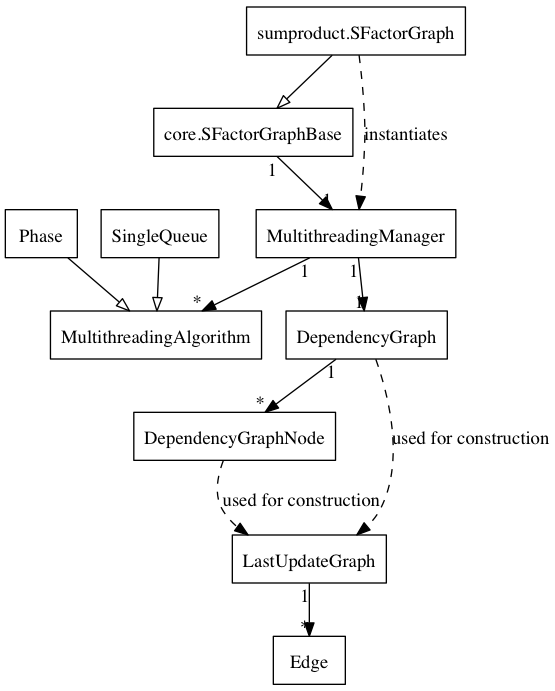
\includegraphics[width=\textwidth,height=\textheight,keepaspectratio]{images/multithreading_classes.png}

\begin{itemize}
\item SFactorGraphBase - This class is contained with in the com.analog.dimple.solvers.core package.  It contains a pointer to the MultithreadingManager and is the class the user interacts with to set the number of threads.
\item sumproduct.SFactorGraph - The sumproduct.SFactorGraph class inherits from the SFactorGraphBase class.  It is responsible for instantiating the MultithreadingManager class.  If it does not instantiate and set this class on it's parent, the SFactorGraphBase class will assume this specific solver does not support multithreading.
\item MultithreadingManager - This class is responsible for switching between various MultithreadingAlgorithms.
\item MultithreadingAlgorithm - This is an abstract class that contains an abstract iterate method.
\item DependencyGraph - This will be described in more detail in the next paragraph.  It contains nodes that represent schedule entries.  It also contains directed edges from Node to Node indicating which schedule entries must be completed before updating a particular schedule entry.
\item DepdendencyGraphNode - Contains a one to one mapping to an IScheduleEntry
\item LastUpdateGraph and Edge - These classes are used by the DependencyGraph initialization code.  
\item Phase - One of the runtime algorithms.  Described in more detail in a later section.
\item SingleQueue - One of the runtime algorithms.  Described in more detail in a later section.
\end{itemize}

\paragraph{Dependency Graph}

Multithreading algorithms require knowledge of the Dimple Schedule.  From a Dimple schedule, we can build a DependencyGraph.  For each ScheduleEntry in a Dimple Schedule, the DependencyGraph contains a list of other ScheduleEntries that must be completed first.

To clarify, we can examine a small graph and its dependency graph.  The following code creates a small FactorGraph with four variables and four factors.

\begin{lstlisting}

N = 2;
fg = FactorGraph();
fg.Scheduler='TreeOrSequentialScheduler';
b = Bit(N);
fh = fg.addFactorVectorized(@(a,b) rand(), b(:,1:end-1),b(:,2:end));
fv = fg.addFactorVectorized(@(a,b) rand(), b(1:end-1,:),b(2:end,:));
for i=1:N
    for j=1:N
        b(i,j).Name = sprintf('B%i_%i',i,j);
    end
end
for i = 1:size(fh,1)
    for j = 1:size(fh,2)
        fh(i,j).Name = sprintf('fh%d_%d',i,j);
    end
end
for i = 1:size(fv,1)
    for j = 1:size(fv,2)
        fv(i,j).Name = sprintf('fv%d_%d',i,j);
    end
end
fg.Solver.getMultithreadingManager().getDependencyGraph().createDotFile('stuff.dot');
fg.Solver.getModelObject().getSchedule()
\end{lstlisting}

We use the TreeOrSequentialScheduler which will produce a more interesting schedule and dependency graph than the FloodingScheduler.  The previous code will display the schedule:

\begin{lstlisting}
ans =
 
FixedSchedule 12
	IScheduleEntry [B1_1] -> 0 -> [fh1_1]
	IScheduleEntry [B1_2] -> 0 -> [fh1_1]
	IScheduleEntry [fh1_1]
	IScheduleEntry [B2_1] -> 0 -> [fh2_1]
	IScheduleEntry [B2_2] -> 0 -> [fh2_1]
	IScheduleEntry [fh2_1]
	IScheduleEntry [B1_1] -> 1 -> [fv1_1]
	IScheduleEntry [B2_1] -> 1 -> [fv1_1]
	IScheduleEntry [fv1_1]
	IScheduleEntry [B1_2] -> 1 -> [fv1_2]
	IScheduleEntry [B2_2] -> 1 -> [fv1_2]
	IScheduleEntry [fv1_2]

 
\end{lstlisting}

From this schedule, the Dependency graph is built:

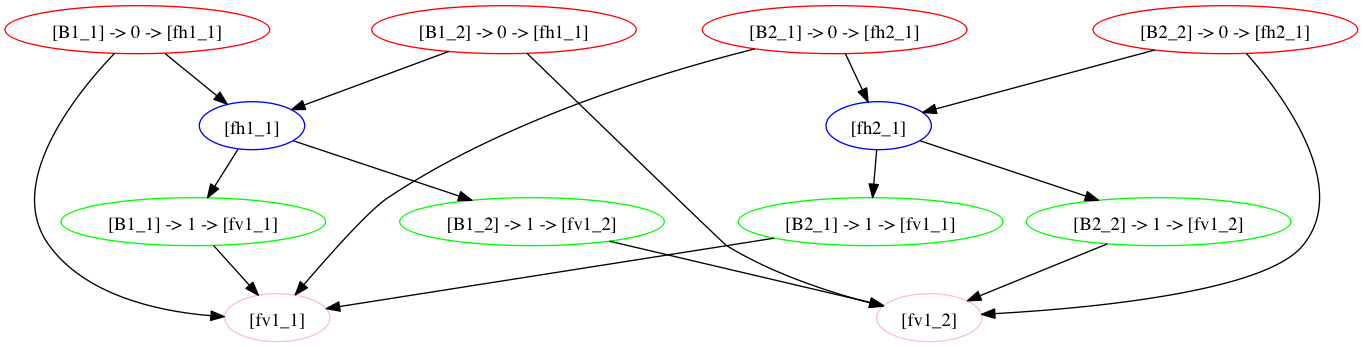
\includegraphics[width=\textwidth,height=\textheight,keepaspectratio]{images/DependencyGraph.png}

Note that the ScheduleEntry for b11 to fh11 has two dependents: fv11 and fh11.  This is because fv11 provides the input to this update and fh11 receives the output from this update.

In addition to building up the list of dependencies, the Dependency Graph will create "phases" (colored red, blue, green and pink in this image).  These phases are used by the PhaseMultithreadingAlgorithm.

\subparagraph{Constructing the DependencyGraph}

The DependendcyGraph uses the LastUpdateGraph and Edge classes to aid in construction.  The following is pseudocode for constructing the DependencyGraph

\begin{lstlisting}
for each entry in schedule
    create new DependencyGraphNode
    for each edge involved in the update
    	see if a previous DependencyGraphNode has read or written this edge (using the LastUpdateEdge)
	if it has
		add this guy to the list of dependents for that guy
		Increment the number of dependencies this guy has
	add this guy to the edge as the last DependencyGraphNode to update the edge
\end{lstlisting}


\paragraph{Runtime algorithms}

Dimple currently provides three multithreading algorithms.
\subparagraph{PhaseMultithreadingAlgorithm}
As previously mentioned, the DependencyGraph contains a list of lists of DependencyGraph nodes.  Each list is known as a phase.  Each phase contains a list of DependencyGraphNodes that contain completely independent IScheduleEntries.  The PhaseMultithreadingAlgorithm operates as:

\begin{lstlisting}
for each phase
	Kick of N threads (user sets N)
	each thread
		pick off num entries in phase / N
		update all of these entries
		when out, try to steal from other queues
		for each other queue
			try to pick off work from that queue
		if no work left, end execution for this thread
\end{lstlisting}

The work stealing improves performance quite a bit.  Also, each thread having its own queue often provides better performance than the SingleQueue algorithms discussed below.  Specifically, when there are many small factors, this algorithm works much better than the following two algorithms.
	
\subparagraph{SingleQueueMultithreadingAlgorithm}
This algorithm uses a single work queue that is initialized with all schedule entries with no dependencies. 

\begin{lstlisting}
for each thread
	take something from the queue (block until we get something)
	if the something is "Poison"
		we're done
		add Poison back to the queue for other threads
		quit this thread
	else
		update the schedule entry
		for each dependent
			decrement the number of dependencies (synchronized)
			if num dependencies is now 0
				add the new DependencyGraphNode to the queue
\end{lstlisting}

This algorithm is slower than the Phase based algorithm in many cases, but does tend to be faster with large factors and a more complex dependency graph.

\paragraph{Profiling}
Dimple contains a few MATLAB profiling scripts in: /dimple/modelers/matlab/tests/performance/threading.  These can be run to determine if multithreading changes affect performance.

\paragraph{Future Direction}
Currently multithreading must be turned on by the user.  In addition, the user is responsible for selecting the algorithm.  In the future it would be good to turn on multithreading by default and allow Dimple to auto tune the threading.

Additionally, we should explore different directions with the threading.  One possibility is to use graph coloring to select subset of phases that would allow one thread to progress into the next phase before the previous phase is complete.

\end{document}  